\documentclass[tikz,border=4pt]{standalone}
\usepackage{pgfplots}\usepgfplotslibrary{groupplots}
\pgfplotsset{compat=1.18}
\definecolor{corba}{HTML}{365FB3}\definecolor{guia}{HTML}{7C3AED}\definecolor{punt}{HTML}{B91C1C}
\begin{document}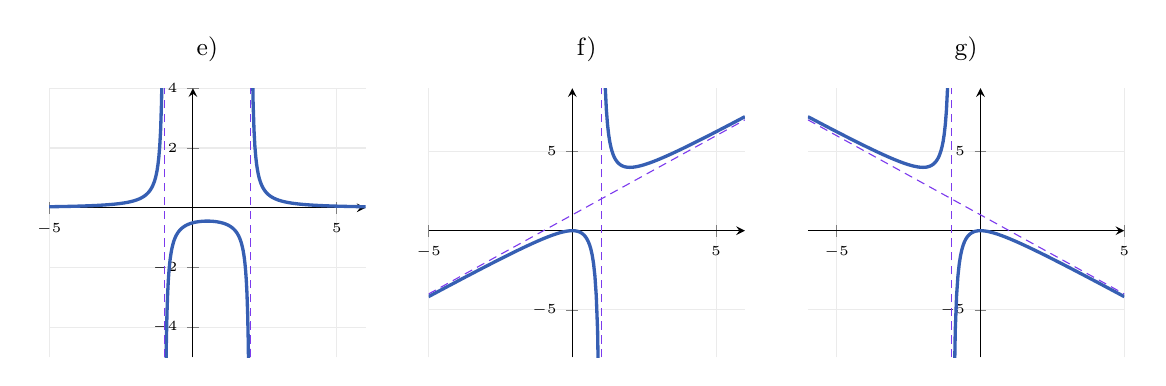
\begin{tikzpicture}
\begin{groupplot}[group style={group size=3 by 1,horizontal sep=0.8cm},
 width=5.6cm,height=5cm,axis lines=middle,grid=major,grid style={black!8},tick label style={font=\tiny},title style={font=\small},samples=130]
\nextgroupplot[title={e)},xmin=-5,xmax=6,ymin=-5,ymax=4]
 \addplot[corba,very thick,domain=-5:-1.03]{1/((x+1)*(x-2))};\addplot[corba,very thick,domain=-.97:1.97]{1/((x+1)*(x-2))};\addplot[corba,very thick,domain=2.03:6]{1/((x+1)*(x-2))};
 \addplot[guia,densely dashed] coordinates {(-1,-5)(-1,4)};\addplot[guia,densely dashed] coordinates {(2,-5)(2,4)};
\nextgroupplot[title={f)},xmin=-5,xmax=6,ymin=-8,ymax=9]
 \addplot[corba,very thick,domain=-5:.97]{x^2/(x-1)};\addplot[corba,very thick,domain=1.03:6]{x^2/(x-1)};
 \addplot[guia,densely dashed] coordinates {(1,-8)(1,9)};\addplot[guia,densely dashed,domain=-5:6]{x+1};
\nextgroupplot[title={g)},xmin=-6,xmax=5,ymin=-8,ymax=9]
 \addplot[corba,very thick,domain=-6:-1.03]{-x^2/(x+1)};\addplot[corba,very thick,domain=-.97:5]{-x^2/(x+1)};
 \addplot[guia,densely dashed] coordinates {(-1,-8)(-1,9)};\addplot[guia,densely dashed,domain=-6:5]{-x+1};
\end{groupplot}\end{tikzpicture}\end{document}
